\documentclass[tikz,border=1mm,10pt]{standalone}
%\usepackage[dvipsnames]{xcolor}
\usepackage{pgfplots}
\pgfplotsset{compat=1.5.1}
\begin{document}
	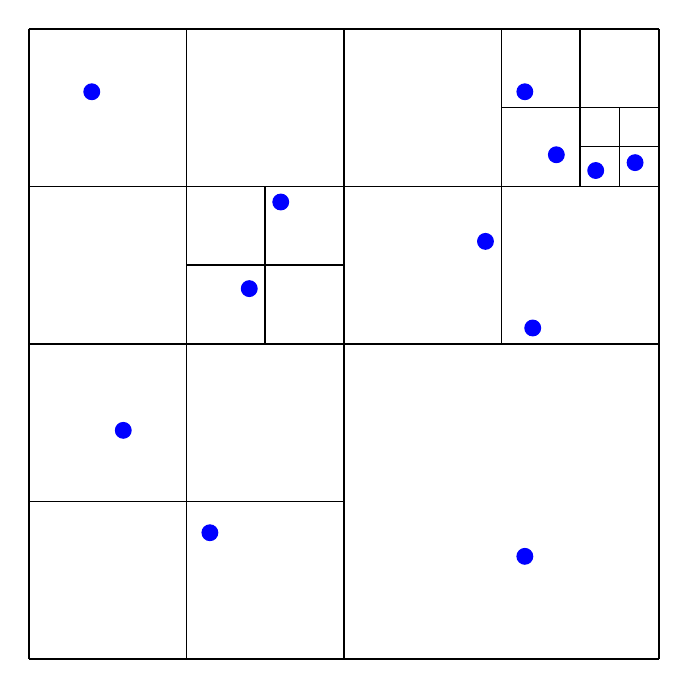
\begin{tikzpicture}[xscale=1,yscale=1,samples=400, transform shape]
	%========
	%Grid
	%========
	\draw[step=4,thick] (0,0) grid (8,8);	%Coarse Grid
	
	\draw[step=2,thin] (0,0) grid (4,4);	%Level 1	
	\draw[step=2,thin] (4,4) grid (8,8);	%Level 1
	\draw[step=2,thin] (0,4) grid (4,8);	%Level 1
	
%	\draw[step=1,thin] (0,2) grid (2,4);	%Level 2
	\draw[step=1,thin] (2,4) grid (4,6);	%Level 2
	\draw[step=1,thin] (6,6) grid (8,8);	%Level 2
	
%	\draw[step=.5,thin] (3,5) grid (4,6);	%Level 3
	\draw[step=.5,thin] (7,6) grid (8,7);	%Level 3

	\draw[blue,fill] (6.3,1.3) circle (.1) ;
	
	\draw[blue,fill] (2.3,1.6) circle (.1) ;
	\draw[blue,fill] (1.2,2.9) circle (.1) ;	
	
	\draw[blue,fill] (0.8,7.2) circle (.1) ;	
	\draw[blue,fill] (3.2,5.8) circle (.1) ;
	\draw[blue,fill] (2.8,4.7) circle (.1) ;
	
	\draw[blue,fill] (5.8,5.3) circle (.1) ;
	\draw[blue,fill] (6.3,7.2) circle (.1) ;
	\draw[blue,fill] (7.2,6.2) circle (.1) ;
	\draw[blue,fill] (7.7,6.3) circle (.1) ;
	\draw[blue,fill] (6.7,6.4) circle (.1) ;		
	\draw[blue,fill] (6.4,4.2) circle (.1) ;
	\end{tikzpicture}
\end{document}